\documentclass[10pt,a4paper]{article}

\usepackage[utf8]{inputenc}		% Configuro la codificación
\input{.command.tex}
% En el siguiente archivo se configuran las variables del trabajo práctico
%% \providecommand es similar a \newcommnad, salvo que el primero ante un 
%% conflicto en la compilación, es ignorado.

% Al comienzo de un TP se debe modificar los argumentos de los comandos

\providecommand{\myTitle}{Trabajo prático de laboratorio} 
\providecommand{\mySubtitle}{Ensayos acústicos de pantallas}

\providecommand{\mySubject}{Acústica (86.57)}
\providecommand{\myKeywords}{UBA, Ingeniería, Control}

\providecommand{\myAuthorSurname}{Lean Cole}
\providecommand{\myTimePeriod}{Año 2019 - 2\textsuperscript{do} Cuatrimestre}

% No es necesario modificar este %%%%%%%%%%%%%%
\providecommand{\myHeaderLogo}{header_fiuba}
%%%%%%%%%%%%%%%%%%%%%%%%%%%%%%%%%%%%%%%%%%%%%%%%

% Si se utilizan listings, definir el lenguaje aquí
\providecommand{\myLanguage}{matlab} 
% Crear los integrantes del TP con el comando \PutMember donde
%%		1) Apellido, Nombre
%%		2) Número de Padrón
%%		3) E-Mail
\providecommand{\MembersOnCover}[0]
{		
		\PutMember{Lean Cole, Micaela}{96364}{leancolem@gmail.com}
}

\providecommand{\myGroupNumber}{25}


\Pagebreaktrue		% Setea si hay un salto de página en la carátula
\Indextrue
\Siunitxtrue			% Si quiero utilizar el paquete, \siunixtrue. Si no \siunixfalse
\Todonotestrue		% Habilita/Deshabilita las To-Do Notes y las funciones \unsure, \change, \info, \improvement y \thiswillnotshow.
\Listingstrue
\Keywordsfalse
\Putgroupfalse		% Habilita/Deshabilita el \myGroup en los headers
\Videofalse
				% Archivo con los comandos globales como Título y autores
%Preambulo para articulo científico de LaTeX

\usepackage[a4paper,left=3cm,right=3cm,bottom=3.5cm,top=3.5cm]{geometry} 	% Configuro la geometría del papel
%\usepackage{microtype}								% Mejora el "spacing" de las palabras
\usepackage[spanish]{babel} 							% Compatibilizo los signos del español
	\addto\captionsspanish{\renewcommand{\tablename}{Tabla}}		%% Redefino nombres preestablecidos por Babel
	\addto\captionsspanish{\renewcommand{\listtablename}{Índice de tablas}}	%% y así en vez de Cuadro dirá Tabla.
\usepackage{amsmath, amsfonts, amssymb}						% Entornos matemáticos, fuentes y símbolos
\usepackage{graphicx}								% Necesario para insertar figuras
\usepackage{fancyhdr}								% Para manipular headers y footers
\usepackage[usenames,dvipsnames]{color}						% \color{color deseado} {lo que querés que tenga color}
\usepackage{subcaption}								% Permite captions del tipo 1a, 1b
\usepackage{multirow}								% Para tablas
\usepackage{float}
\usepackage{mathtools}

% Para video
\ifVideo
	\usepackage{media9}
	\addmediapath{./../reportes/}
\fi

%\usepackage{times}
%\usepackage{mathtools}
%\usepackage{upgreek} % letras griegas sin cursiva
%\usepackage{cancel}
\usepackage{rotating}
\usepackage{tikz}
\usepackage{pgfplots}
%	\pgfplotsset{compat=1.12}
	\usetikzlibrary{plotmarks}% matlab2tikz
\usepackage{grffile}% matlab2tikz 
	\usetikzlibrary{calc,patterns,decorations.pathmorphing,decorations.markings}

\ifListings
	\usepackage{listings}

	\providecommand{\lstinputpath}[1]{\lstset{inputpath=#1}}

%	\input{.lst_default.tex}
	\input{.lst_matlab.tex}
%	\input{.lst_c.tex}
%	\input{.lst_c++.tex}
	
% 	\input{.lst_pseudocode.tex}


\fi

\ifSiunitx
\usepackage{siunitx}											% Unidades: \SI {cantidad} {\unidad} (necesita texlive-science)
	\sisetup{load-configurations = abbreviations}							% Habilita poner \cm en vez de \centi\metre
%	\sisetup{output-decimal-marker = {,}}									% Cambia los puntos decimales por comas
	\sisetup{per-mode = fraction}											% Pone las unidades como fracción
	\sisetup{quotient-mode = fraction}										
\fi


\ifTodonotes
\usepackage{xargs}
\usepackage[colorinlistoftodos,prependcaption,textsize=tiny]{todonotes}


	\newcommandx{\juan}[2][1=]{\todo[linecolor=blue,backgroundcolor=blue!25,bordercolor=blue,#1]{#2}}
	\newcommandx{\mcoul}[2][1=]{\todo[linecolor=green,backgroundcolor=green!25,bordercolor=green,#1]{#2}} % OliveGreen
	\newcommandx{\improvement}[2][1=]{\todo[linecolor=orange,backgroundcolor=orange!25,bordercolor=orange,#1]{#2}}
	\newcommandx{\unsure}[2][1=]{\todo[linecolor=red,backgroundcolor=red!25,bordercolor=red,#1]{#2}}
	\newcommandx{\thiswillnotshow}[2][1=]{\todo[disable,#1]{#2}}
\fi


\usepackage{booktabs}														% Permite hacer tablas sin separadores en el medio
\usepackage{placeins}														
		\let\Oldsection\section												%% Permite que los flotantes (como figuras) no aparezcan
	\renewcommand{\section}{\FloatBarrier\Oldsection}						%% antes o después de su sección correspondiente.
		\let\Oldsubsection\subsection
	\renewcommand{\subsection}{\FloatBarrier\Oldsubsection}		
		\let\Oldsubsubsection\subsubsection
	\renewcommand{\subsubsection}{\FloatBarrier\Oldsubsubsection}
\usepackage{hyperref}														% Debe ser agregado al final del preambulo

\hypersetup
{    bookmarks=true,         % show bookmarks bar?
     unicode=false,          % non-Latin characters in Acrobat’s bookmarks
     pdftoolbar=true,        % show Acrobat’s toolbar?
     pdfmenubar=true,        % show Acrobat’s menu?
     pdffitwindow=false,     % window fit to page when opened
     pdftitle={\myTitle},    		 % title
     pdfauthor={\myAuthorSurname},   % author
	 pdfcreator={\myAuthorSurname},	 % creator = author
     pdfsubject={\mySubject},		 % subject of the document
     pdfkeywords={\myKeywords},
     colorlinks=true,        % false: boxed links; true: colored links
     linkcolor=black,        % color of internal links (change box color with linkbordercolor)
     citecolor=black,        % color of links to bibliography
     filecolor=magenta,      % color of file links
     urlcolor=cyan           % color of external links
}

%Configuro la pagina con los encabezaos y pies de paginas
\pagestyle{fancy}										% Para agregar encabezados y pie de paginas	
\lhead{\mySubject}										% Encabezado izquierdo
\rhead{\includegraphics[scale=0.15]{\myHeaderLogo}} 	% Encabezado derecho (logo de la FIUBA)	
\ifPutgroup
\chead{\texttt{Alumno Nº\myGroupNumber} }%\\ \textit{\footnotesize{\myTimePeriod}}}
\fi				

%% Este archivo contiene las funciones auxiliares para escribir en LaTeX
%% Dichas funciones resuelven la sintaxis de generar figuras, por ejemplo,
%% dejando el código más compacto y facilitando la corrección del mismo.



% Comando para graficar eps. 1er arg, escala. 2do, ruta. 3ro, caption. 4to, label.
\providecommand{\HgraficarEPS}[4]{
			\begin{figure}[h!]
				\centering
					\scalebox{#1}{\input{#2}}
					\caption{#3}
					\label{#4}
			\end{figure}

}

\providecommand{\HgraficarPNG}[4]{
			\begin{figure}[H]
				\centering
					\includegraphics[scale=#1]{#2}
					\caption{#3}
					\label{#4}
			\end{figure}

}


% Comando para graficar eps en el lugar previsto.
\providecommand{\graficarEPS}[4]{
			\begin{figure}[h]
				\centering
					\scalebox{#1}{\input{#2}}
					\caption{#3}
					\label{#4}
			\end{figure}

}

\providecommand{\graficarPNG}[4]{
			\begin{figure}[h]
				\centering
					\includegraphics[scale=#1]{#2}
%		\includegraphics[width=1.0\textwidth,keepaspectratio]{#1}
					\caption{#3}
					\label{#4}
			\end{figure}

}

\providecommand{\graficarPDF}[3]{
			\begin{figure}[h!]
				\centering
		\includegraphics[width=1.0\textwidth,keepaspectratio]{#1}
					\caption{#2}
					\label{#3}
			\end{figure}

}


\providecommand{\graficarPDFwide}[3]{
			\begin{figure}[h!]
				\centering
		\includegraphics[scale=0.5,trim={6,5cm 0 0 0}]{#1}
					\caption{#2}
					\label{#3}
			\end{figure}

}

\providecommand{\graficarPDFa}[4]{
			\begin{figure}[h!]
				\centering
				\includegraphics[scale=0.5,trim={#1}]{#2}
					\caption{#3}
					\label{#4}
			\end{figure}

}



\providecommand{\underuparrow}[2]{\underset{\underset{#2} \uparrow} #1 }

\providecommand{\cltext}[2]{\color{#1}{\huge{#2}}}

\providecommand{\cstext}[2]{\color{#1}{\large{#2}}}

\providecommand{\vect}[1]{\boldsymbol{#1}}
\providecommand{\dvect}[1]{\dot{\boldsymbol{#1}}}
\providecommand{\ddvect}[1]{\ddot{\boldsymbol{#1}}}
\providecommand{\dd}{\mathrm{d}}
\providecommand{\deriv}[2]{\frac{d#1}{d#2}}
\providecommand{\ilap}{\mathcal{L}^{-1}}
\providecommand{\lap}{\mathcal{L}}

		% Se proveen un conjunto de funciones extras

% Defino el path de los includegraphics
\graphicspath{{./Figuras/}}		% Directorio que contiene los graficos

% Defino el path para los input de .tex y de .eps
\makeatletter
\def\input@path{{./Figuras/}{./Secciones/}{./Cover_page/}}
\makeatother

% Defino el path del listings
\ifListings
%% Cambiar el nombre de la carpeta si se utilizan Listings
	\lstinputpath{{../Matlab/}}
\fi

\definecolor{myred}{rgb}{0.5,0,0}
\definecolor{mygreen}{rgb}{0,0.5,0}

\renewcommand{\thesubsubsection}{\thesubsection.\alph{subsubsection}}

\pagestyle{fancy}
\renewcommand{\sectionmark}[1]{\markboth{}{\thesection\ \ #1}}
\lhead{}
\chead{}
\rhead{\rightmark}
\lfoot{Acústica (86.57)}
\cfoot{}
\rfoot{P\'agina \thepage\ de 13}

\begin{document}
		% Carátula (formal o simple,_formal o _simple respectivamente) con Resumen
		% incluido e Índice (si es necesario configurar en config.tex) del informe
		\begin{titlepage}

\thispagestyle{empty}

\begin{center}

\includegraphics[scale=0.3]{fiuba}\\
\large{\textsc{Universidad de Buenos Aires}}\\
\large{\textsc{Facultad De Ingeniería}}\\
\small{A\~no 2019 - 2\textsuperscript{do} Cuatrimestre}
\end{center}

\begin{center}
\Large{\underline{\textsc{Acústica (86.57)}}}

\vspace*{1.5cm}

\textbf{\begin{LARGE}
Acondicionamiento acústico interior de una sala para conferencias
\end{LARGE}}
\end{center}

\vspace*{3cm}

\begin{tabbing}
\hspace{2cm}\=\+
\\
	ALUMNOS:\hspace{-1cm}\=\+\hspace{1cm}\=\hspace{6cm}\=\\
		Lean Cole, Micaela \>\>\#\ 96364\\
		\>\footnotesize{$<$mleancole@icloud.com$>$}			
\end{tabbing}
\end{titlepage}

%	\setcounter{page}{1}
	
	% Hago que las páginas se comiencen a contar a partir de aquí:
% Pongo el índice en una página aparte:
\tableofcontents
%\listoffigures
%\listoftables
\newpage
\setcounter{page}{1}
%----------------------------- Consigna del TP --------------------------------
%\marginsize{1cm}{1cm}{1cm}{1cm}

%	\begin{center}{\Large{\textbf{Introducción}}}\end{center}

\section{Introducción}
	\input{0_introducción}

\section{Etapa 1: determinación del volumen del recinto}
	\subsection{Objetivo}

	En esta primera etapa se busca calcular el volumen de la sala, y planificar el esquema de planta de la misma. En concreto, se debe:

	\begin{itemize}
		\item Especificar la altura elegida del recinto;
		\item Especificar la capacidad de la sala (cantidad de butacas que se instalarán);
		\item Realizar un esquema de planta: ubicación de butacas, oradores, puertas, pasillos, etc;
		\item Indicar las dimensiones más relevantes: pasillos, puertas, espacio para oradores, butacas, separación entre butacas, etc.
	\end{itemize}

\subsection{Importancia de las dimensiones del recinto}

Un factor importante que afecta el comportamiento de los recintos son sus \textsc{modos de resonancia}:

\begin{itemize}
	\item Cuando el sonido se refleja entre dos superficies paralelas, se producen interferencias constructivas y destructivas, dando lugar a la formación de ondas estacionarias o \textit{modos propios de la sala};
	\item Es una característica propia de cada sala y el efecto que produce se denomina \textit{coloración}. Es más común en recintos pequeños, como los estudios de grabación, por ejemplo.
\end{itemize}

Un \textit{modo propio} es una onda estacionaria generada en el interior de una sala. Se producen por la interacción entre las ondas incidentes y reflejadas dentro del recinto. Cada modo está asociado a una frecuencia (frecuencia propia).\\

Si la distancia entre dos superficies paralelas de una sala es igual a media longitud de onda (d = $\lambda/2)$, se generará una onda que permanecerá estacionaria reflejándose entre las dos superficies paralelas, perdiendo paulatinamente energía acústica. Estos refuerzos ocurrirán fundamentalmente para tres frecuencias básicas correlacionadas con las dimensiones del recinto (largo, ancho y altura) y para sus múltiplos.\\

Según la cantidad de superficies que intervengan, los modos podrán ser \textsc{axiales} (se establecen entre dos superficies), \textsc{tangenciales} (entre cuatro superficies) u \textsc{oblicuos} (entre las seis superficies del recinto).\\

El cálculo de frecuencias de modos de resonancia o modos propios se realiza de acuerdo a la siguiente expresión:

\begin{equation}
	f_{modos} = \frac{c}{2}\,\sqrt{\left(\frac{p}{L} \right)^2 + \left(\frac{q}{W} \right)^2 + \left(\frac{r}{H} \right)^2},\quad \forall\, p,q,r \,\in \mathbb{Z}
\end{equation}

Donde:

\begin{itemize}
	\item $f_m$: frecuencia del modo de resonancia;
	\item $c$: velocidad del sonido, en m/s;
	\item $p,\,,\,r$: números enteros que denotan el número de medias longitudes de onda en las 3 direcciones (0, 1, 2,...);
	\item $L,\,W,\,H$: las dimensiones del recinto, en m.
\end{itemize}

Según el valor que tomen p, q y r en la expresión anterior:

\begin{itemize}
	\item Si uno es distinto de cero, son modos \textsc{axiales};
	\item Si dos son distintos de cero, son modos \textsc{tangenciales};
	\item Si tres son distintos de cero, son modos \textsc{oblicuos}.
\end{itemize}

\subsection{Aplicación del criterio de Bonello}

Bonello contempla todos los modos presentes, fijando el análisis sobre la base de porcentajes de la frecuencia modal y no a distancias fijas.\\ 

Primero, se calculan todas las frecuencias de modos propios del recinto que estén por debajo de la \textsc{frecuencia de Schroeder}, que está dada por la siguiente expresión:

\begin{equation}
	f_s = 1893\,\sqrt{\frac{TR}{V}}
\end{equation}

Luego, se divide el espectro en tercios de octava hasta la $f_s$ obtenida, pues el análisis por tercios satisface a la discriminación de frecuencias del oído.\\

El último paso es calcular y graficar la \textit{densidad de modos} (cantidad de modos por cada tercio de octava).\\

Finalmente, para decidir si cumple con el Criterio de Bonello, se debe cumplir que:

\begin{enumerate}
	\item La curva de densidad de modos debe ser monótonamente creciente, o a lo sumo tener la misma cantidad de modos en dos tercios de octava sucesivos;
	\item No deben existir modos dobles y, si los hubiera, se los tolera en tercios de octava con densidad de modos mayor que cinco.
\end{enumerate}


%% Valor aceptable en ambientes desocupados (sin personas) / criterio NC recomendado para sala de conferencias: NC25-30.

\subsection{Cálculos}

Para aplicar el criterio, se acude a alguna herramienta online de cálculo; en este caso, se usó \texttt{amroc: the room mode calculator}\footnote{https://amcoustics.com/tools/amroc}. Es muy útil para ver cómo varía la distribución de los modos de acuerdo a las dimensiones del salón.\\

\HgraficarPNG{0.45}{amroc_parámetros.png}{Parámetros finales usados para aplicar el criterio de Bonello.}{amroc_parámetros}

Primero se fijaron las dimensiones de ancho y largo del recinto, que son dato; luego, de indicó la norma correspondiente para tener el \texttt{RT60} adecuado (en este caso, se sabe que es una sala destinada a la palabra, por lo que se seleccionó \textit{Speech}). La dimensión restante, que es la altura, se fue variando entre los límites de lo que se considera una altura sensata para una sala de conferencias, en cuanto a términos de arquitectura. Luego de consultar varias fuentes y de dimensionar el recinto con una herramienta CAD, se llegó a un valor de altura \texttt{H = 4.9m}. Si bien, una altura más baja podría ser considerada un poco más apropiada visualmente, esta altura elegida cumple perfectamente con el criterio de Bonello, y tampoco es tan grande como para ser considerada desproporcionada.

Con la altura elegida, el gráfico de Bonello que muestra la herramienta se ve así:

\HgraficarPNG{0.7}{amroc_bonello.png}{Gráfico de la cantidad de modos por tercio de octava que provee la herramienta.}{amroc_bonello}

A partir de este gráfico, se puede concluir en que el criterio se cumple para este valor de altura elegido, ya que es monótonamente creciente (sólo hay dos bandas de octava con la misma cantidad de modos, pero cumplen con el criterio por ser consecutivas).

\HgraficarPNG{0.55}{amroc_adicional.png}{Información adicional que provee la herramienta.}{amroc_adicional}

En la Figura \ref{amroc_adicional}, se puede ver que gracias a esta herramienta, también se obtiene el cálculo del volumen y la superficie del recinto, así como el valor de la frecuencia de Schroeder y la distancia crítica (que sirve para el análisis de la segunda etapa).\\

La frecuencia de Schroeder se puede calcular como:

\begin{equation}
	f_s = 1893\,\sqrt{\frac{TR}{V}} = 1893\,\sqrt{\frac{0.75\,s}{438.35\,m^3}} \approx 78 Hz
\end{equation}

	A diferencia del valor calculado, la herramienta provee un valor de $f_s =$ \SI{83}{\Hz}, que resulta de calcular la expresión de arriba con un factor de $2000$ en vez de $1893$; esta aproximación se suele utilizar.\\

	Recortando entonces el rango de frecuencias de interés, se calcularon un total de 45 modos, que se verán detallados en la siguiente Tabla (repartida en las Figuras \ref{amroc_tabla_1}, \ref{amroc_tabla_2}). Para cada modo, se indica la frecuencia eel mismo, si es axial, tangencial u oblicuo, y la combinación de los parámetros p, q, r que logran dicho modo:
	
	\begin{figure}[H]
		\centering
		\begin{subfigure}{.5\textwidth}
  			\centering
  			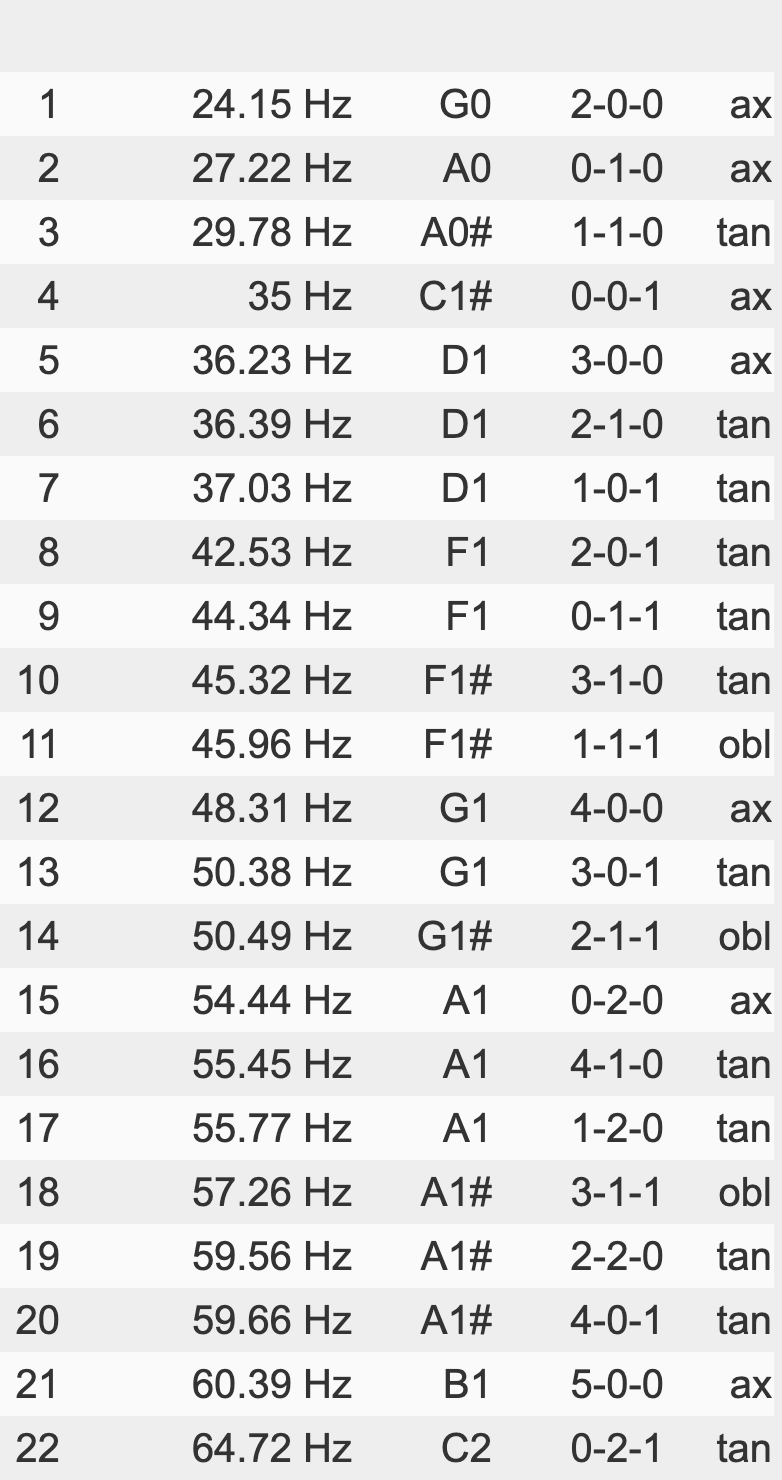
\includegraphics[width=0.8\linewidth]{amroc_tabla_1.png}
  			\caption{Rango de frecuencias 24.1-65.4Hz}
  			\label{amroc_tabla_1}
		\end{subfigure}%
		\begin{subfigure}{.5\textwidth}
  			\centering
  			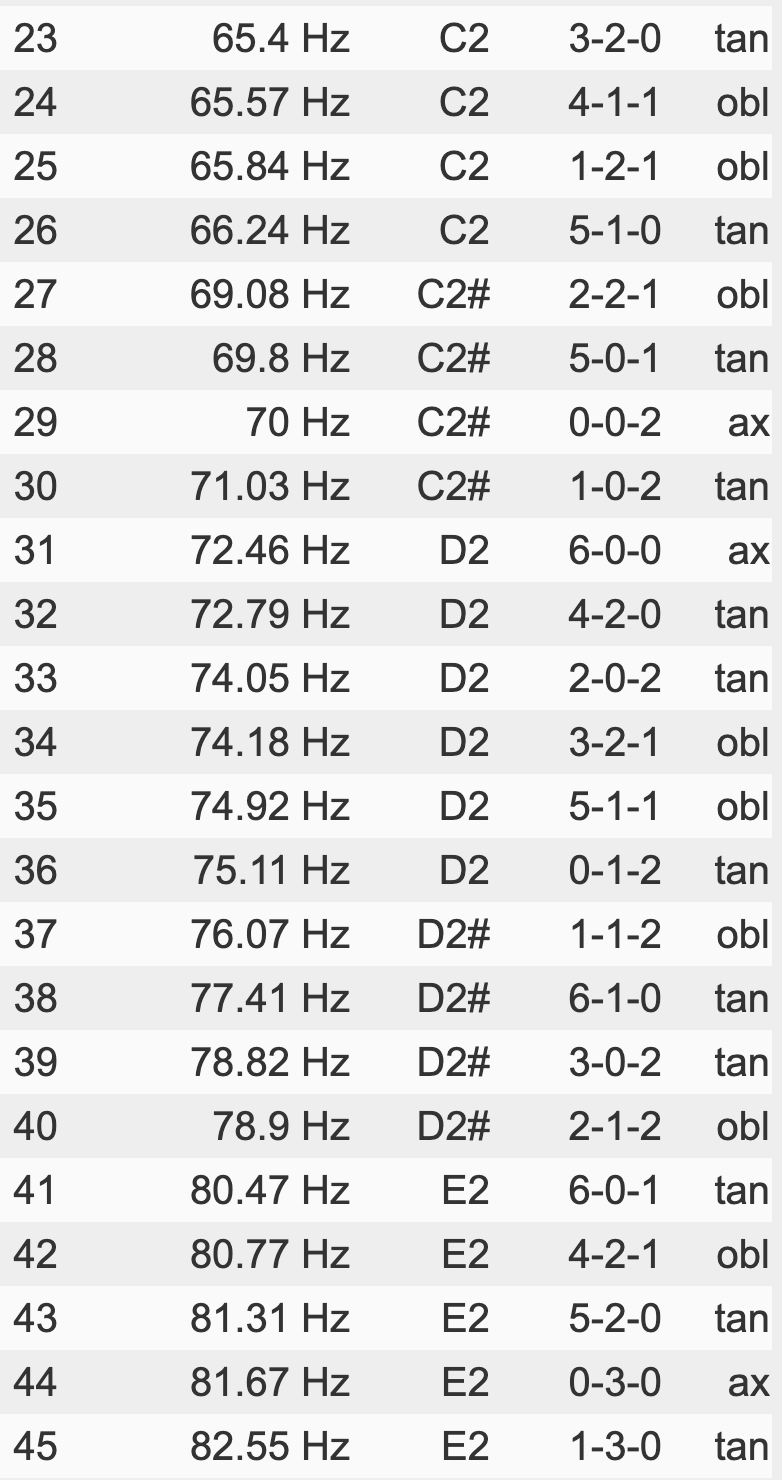
\includegraphics[width=0.8\linewidth]{amroc_tabla_2.png}
  			\caption{Rango de frecuencias 65.5-82.55Hz.}
  			\label{amroc_tabla_2}
		\end{subfigure}
		\caption{Tabla con la información detallada de todos los modos analizados entre las frecuencias de interés.}
		\label{amroc_tablas}
	\end{figure}

En estas tablas, se puede comprobar que se cumple con el segundo criterio de Bonello, ya que no existen modos iguales.\\

A partir de los datos relevados de estas tablas, se graficó la cantidad de modos por tercio de octava, para comprobar que resultara como en la simulación, y se obtuvo lo siguiente:

\HgraficarPNG{0.4}{curva_bonello.png}{Esquema de la planta que será utilizada como una sala de conferencias.}{curva_bonello}

Se pueden notar algunas diferencias con la curva que provee la herramienta, pero lo importante es que sigue cumpliendo con el criterio de Bonello: es monótonamente creciente (cumple con el primer criterio de Bonello). Las diferencias se dan por la cantidad de modos que considera la herramienta: toma 29 modos, mientras que en mi caso tomo los 45 modos que me provee la tabla.\\

Luego de estos cálculos, se presentan una tabla con los parámetros de interés para el recinto:

		\begin{table}[h!]
			\centering
			\begin{tabular}{cc}
			\toprule
			\textbf{Largo} & \textbf{\SI{14.2}{\m}}\\
			\midrule
			\textbf{Ancho} & \textbf{\SI{6.3}{\m}}\\
			\midrule
			\textbf{Alto} & \textbf{\SI{4.9}{\m}}\\
			\midrule
			\textbf{Volumen} & \textbf{\SI{438.354}{\cubic\m}}\\
			\midrule
			\textbf{Superficie} & \textbf{\SI{379.82}{\square\m}}\\
			\midrule
			\textbf{Frecuencia de Schröder} & \textbf{\SI{83}{\Hz}}\\
			\midrule
			\textbf{Tiempo de reverberación} & \textbf{\SI{0.75}{\s}}\\
			\midrule
			\textbf{Distancia crítica} & \textbf{\SI{1.38}{\m}}\\
			\bottomrule
			\end{tabular}
		\end{table}

Para entender mejor las dimensiones, se plasman los datos en una tabla:

		\begin{table}[h!]
			\centering
			\begin{tabular}{c c}
			\toprule
			\textbf{Ancho de las butacas} & \textbf{$0.54m$}\\
			\midrule
			\textbf{Profundidad de butaca} & \textbf{$0.6m$}\\
			\midrule
			\textbf{Distancia entre filas (de respaldo a respaldo)} & \textbf{$0.9m$}\\
			\midrule
			\textbf{Ancho del pasillo} & \textbf{$0.96m$}\\
			\midrule
			\textbf{Ancho de las puertas} & \textbf{$1.76m$}\\
			\midrule
			\textbf{Distancia entre la última fila y la pared} & \textbf{$1.0m$}\\
			\bottomrule
			\end{tabular}
		\end{table}

Con el esquema de la planta resultante de la Figura \ref{esquema_planta}, se comprueba que pueden entrar \textsc{110 butacas} organizadas en 11 filas de 10 butacas cada una, separadas a la mitad por un pasillo de un ancho suficiente para que la gente transite con mayor comodidad. Detrás de la última fila, se deja un espacio de 1m en caso de querer colocar sillas de ruedas. Además, se incluye una puerta extra trasera para mayor seguridad de evacuación en caso de emergencias; ambas puertas tienen un ancho suficiente para que circule el caudal de gente que entra en la sala, sin generarse atascamientos.\\

\HgraficarPNG{0.45}{esquema_planta}{Esquema de la planta que será utilizada como una sala de conferencias.}{esquema_planta}


\section{Etapa 2: diseño de tratamiento acústico para la sala}
	\subsection{Objetivo}

	Para la segunda etapa, se desea calcular los tiempos de reverberación óptimos y diseñar el tratamiento acústico de la sala, teniendo en cuenta que la misma va a ser utilizada para la palabra. También se requiere calcular la inteligibilidad de palabra.

%%%% 1) Trev optimos dado V y destino, y banda de tolerancia 
%%%% 2) Trev sala desocupada, en octavas entre 125 y 4k
%%%% 3) Porcentaje de ocupación elegido para el cálculo
%%%% 4) Cálculo TR considerando el criterio de ocupación elegido
%%%% 5) Lista de materiales para ese TR (tipo, cantidad, ubicación)
%%%% 6) Trev logrados con diseño final y el estado de ocupación elegido
%%%% 7) Analizar si todas las filas se encuentran a partir de la distancia crítica
%%%% 8) Analizar la importancia de cumplir esta condición en tal recinto
%%%% 9) Cálculo de IL
%%%% 10) Esquema final de la planta si hubo variación

\subsection{Cálculo del tiempo de reverberación óptimo}

	Dados el volumen y el destino, se presenta en la Tabla \ref{tabla:tr_óptimo} el tiempo de reverberación óptimo calculado para cada  octava, entre los \SI{125}{\Hz} y los \SI{4}{\k\Hz}, junto con sus bandas de tolerancia (elegida como criterio de diseño).
	
		\begin{table}[h!]
			\centering
			\resizebox{\textwidth}{!} & \textbf{TR\textsubscript{o}} & \textbf{TR\textsubscript{o} + 20\%}\\
			\midrule
			\textbf{125} & \textbf{$0.41 + 0.26\,\log_{10}\,V$} & \SI{0.877}{\s} & \SI{1.097}{\s} & \SI{1.316}{\s}\\
			\midrule
			\textbf{250} & \textbf{$0.32 + 0.21\,\log_{10}\,V$} & \SI{0.699}{\s} & \SI{0.875}{\s} & \SI{1.050}{\s}\\
			\midrule
			\textbf{$\geq$500} & \textbf{$0.28 + 0.18\,\log_{10}\,V$} & \SI{0.604}{\s} & \SI{0.756}{\s} & \SI{0.907}{\s}\\
			\bottomrule
			\end{tabular}
			}
			\caption{Tiempo de reverberación óptimo calculado, junto con sus respectivas bandas de tolerancia, en función de la frecuencia.}
			\label{tabla:tr_óptimo}
		\end{table}
	
	Cabe destacar que existen diversos criterios de diseño (basados en modelos matemáticos empíricos) y no hay uniformidad de opinión entre los autores de la bibliografía especializada. Se desea que el tiempo de reverberación calculado para esta sala se encuentre dentro del límite de tolerancia del $20\%$ del valor de este tiempo de reverberación óptimo obtenido.

\subsection{Selección de materiales}

	Se elige el tipo de material con que estarán construidas las superficies interiores del recinto (la dimensión de las puertas y butacas elegidas está detallada en la Parte I del informe). Los datos de los coeficientes de absorción se obtienen a partir de tablas construidas por Leo Beranek, facilitadas por la cátedra:
	
		\begin{table}[H]
			\centering
%			\resizebox{\textwidth}{!}{%
			\begin{tabular}{ccc}
			\toprule
			\textbf{Tipo de superficie} & \textbf{Material} & \textbf{Superficie total}\\
			\midrule
			Piso & Parqué pegado & \SI{89.46}{\square\m}\\
			\midrule
			Techo & Hormigón & \SI{89.46}{\square\m}\\
			\midrule
			Pared & Papel pintado & \SI{193.508}{\square\m}\\
			\midrule
			Puerta & Madera maciza & \SI{7.392}{\square\m}\\
			\bottomrule
			\end{tabular}
%			}
			\caption{Tipos de materiales elegidos para las superficies interiores de la sala y la superficie que cubre cada uno.}
			\label{tabla:superficies}
		\end{table}
		
		Los cálculos de la Tabla \ref{tabla:superficies} se realizan teniendo en cuenta que el piso y el techo cubren la misma superficie, de \texttt{\SI{14.2}{\m}$\times$\SI{6.3}{\m} = \SI{89.46}{\square\m}} cada uno; las puertas tienen una superficie de \texttt{2$\times$\SI{1.76}{\m}$\times$\SI{2.10}{\m} = \SI{7.392}{\square\m}} entre las dos; las paredes se calculan teniendo en cuenta que son 2 pares de superficies iguales menos la superficie de las puertas, es decir \texttt{2$\times$\SI{14.2}{\m}$\times$\SI{4.9}{\m} + 2$\times$\SI{6.3}{\m}$\times$\SI{4.9}{\m} - \SI{7.392}{\square\m} = \SI{193.508}{\square\m}}.\\
		
		Para los materiales elegidos, se informa en la Tabla \ref{tabla:coeficientes_sola} sus coeficientes de absorción sonora en cada banda de frecuencia de interés:
		
			\begin{table}[H]
			\centering
%			\resizebox{\textwidth}{!}{%
			\begin{tabular}{@{}ccccccc@{}}
				 & \multicolumn{6}{c}{\textbf{Coeficiente de absorción ($\alpha$)}}\\ \toprule
				\textbf{Frecuencia (Hz)} & \textbf{125} & \textbf{250} & \textbf{500} & \textbf{1k} & \textbf{2k} & \textbf{4k}   \\ \midrule
					Piso                & 0.03 & 0.04 & 0.08 & 0.12 & 0.12 & 0.17 \\ \midrule
					Techo               & 0.01 & 0.01 & 0.02 & 0.02 & 0.05 & 0.07 \\ \midrule
					Pared               & 0.01 & 0.02 & 0.04 & 0.10 & 0.20 & 0.30 \\ \midrule
					Puerta              & 0.05 & 0.11 & 0.10 & 0.09 & 0.08 & 0.10 \\ \bottomrule
			\end{tabular}%
%			}
			\caption{Coeficientes de absorción de los materiales de la sala.}
			\label{tabla:coeficientes_sola}
		\end{table}
		
		A partir de los datos de las Tablas \ref{tabla:superficies} y \ref{tabla:coeficientes_sola}, el área equivalente del recinto se calcula según la siguiente expresión:
		
		\begin{equation}
			A_{sala_{sola}} = A_{piso} + A_{techo} + A_{paredes} + A_{puertas}
		\end{equation}
		
		Las áreas equivalentes de las superficies se calculan a partir del producto entre la superficie y el coeficiente de absorción. Con este valor dado para cada octava considerada, se calcula el tiempo de reverberación según:

		\begin{equation}
			TR_{sala_{sola}} = 0.161 \, \frac{V}{A_{sala_{sola}}}
		\end{equation}
		
		En la Tabla \ref{tabla:tr_finales_sola} se muestra el tiempo de reverberación resultante en cada banda de frecuencia para la sala vacía y sin muebles (mesa de oradores, butacas y tarimas):
		
		\begin{table}[H]
			\centering
%			\resizebox{\textwidth}{!}		& 0.878 & 0.700 & 0.605 & 0.605 & 0.605 & 0.605 \\ \cmidrule{2-8}
					& \textbf{Óptimo}				& 1.097 & 0.875 & 0.756 & 0.756 & 0.756 & 0.756 \\ \cmidrule{2-8}
					& \textbf{Óptimo + 20\%}		& 1.316 & 1.050 & 0.907 & 0.907 & 0.907 & 0.907 \\ \cmidrule{2-8}
					& \textbf{Sala vacía y sin muebles}				& 11.996 & 7.708 & 4.050 & 2.169 & 1.295 & 0.879 \\\bottomrule
			\end{tabular}%
%			}
			\caption{Tabla de tiempos de reverberación de la sala sin muebles.}
			\label{tabla:tr_finales_sola}
		\end{table}
		
		Se grafican los tiempos calculados en la Figura \ref{TR_sola}:
		
		\HgraficarPNG{0.94}{TR_sola.png}{Curvas del tiempo de reverberación obtenido y del óptimo en función de la frecuencia, para la sala vacía y sin muebles.}{TR_sola}
		
		Se puede ver que, especialmente para el rango de frecuencias entre los \SI{100}{\Hz} y \SI{2}{k\Hz}, el tiempo de reverberación obtenido con la colocación de los materiales del techo, piso y paredes, pero sin muebles, se aleja considerablemente del tiempo óptimo. Para obtener un valor más cercano al deseado, se necesitan tiempos de reverberación más cortos, lo que implica mayores áreas equivalentes de absorción para cada octava; ese área equivalente resultante se logra agregando y modificando los muebles de la sala.\\
		
%%%%%%%%%%%%%%%%%% MUEBLES: BUTACAS Y MESA
		
		En la Tabla \ref{tabla:muebles} se detallan los muebles usados para la sala; el índice \textit{(2)} en las butacas se agrega para diferenciarla de la otra butaca que se provee en la tabla de datos del enunciado. La cantidad de butacas vacías y butacas ocupadas varía para cada caso de porcentaje de ocupación, pero en todos los casos suman 113 entre las dos, que es el total de asientos de espectadores y oradores de la sala. Aquí se muestra el caso para un 75\% de ocupación:

		\begin{table}[H]
			\centering
%			\resizebox{\textwidth}{!}{%
			\begin{tabular}{ccc}
			\toprule
			\textbf{Tipo de mueble} & \textbf{Material} & \textbf{Cantidad}\\ \midrule
			Butaca desocupada & Tapizada (2)& 28\\ \midrule
			Butaca ocupada & Tapizada (2)& 85\\ \midrule
			Mesa & Madera & 1\\ \bottomrule
			\end{tabular}
%			}
			\caption{Tipos y cantidades de materiales elegidos para los muebles de la sala.}
			\label{tabla:muebles}
		\end{table}
		
		Se puede ver que las superficies se definen con su coeficiente de absorción, mientras que los objetos puntuales se definen con su área equivalente de absorción sonora, sin considerar la superficie de los mismos, como en la Tabla \ref{tabla:coeficientes_muebles}:
		
		\begin{table}[H]
			\centering
%			\resizebox{\textwidth}{!}{%
			\begin{tabular}{@{}ccccccc@{}}
					& \multicolumn{6}{c}{\textbf{Área equivalente de abs ($A_{eq}$)}}\\ \toprule
				\textbf{Frecuencia (Hz)} & \textbf{125} & \textbf{250} & \textbf{500} & \textbf{1k} & \textbf{2k} & \textbf{4k}   \\ \midrule
					Butaca desocupada   & 0.12 & 0.23 & 0.27 & 0.30 & 0.33 & 0.33 \\ \midrule
					Butaca ocupada      & 0.12 & 0.25 & 0.42 & 0.46 & 0.48 & 0.40 \\ \midrule
					Mesa                & 0.02 & 0.02 & 0.02 & 0.02 & 0.02 & 0.02 \\ \bottomrule
			\end{tabular}%
%			}
			\caption{Áreas equivalentes de absorción de los muebles de la sala.}
			\label{tabla:coeficientes_muebles}
		\end{table}

\subsection{Porcentaje de ocupación}

	Se debe elegir un porcentaje de ocupación con el que se desea lograr los tiempos de reverberación óptimos en el proyecto. Para este proyecto, se decide elegir un porcentaje del $75\%$\footnote{Un buen criterio puede ser elegir un p\% entre 70\% y 80\%, para tener en cuenta que la sala no suene \textit{muy reverberante}, aunque no esté completamente ocupada.}, que equivale a \texttt{85 butacas} ocupadas (se contemplan las 110 butacas de oyentes más 3 butacas para los oradores).\\
	
	Con esto dicho, se contemplan 3 casos al tiempo de analizar los tiempos de reverberación de la sala:
	
	\begin{itemize}
		\item 0\% ocupación: 113 butacas desocupadas y 0 butacas ocupadas;
		\item 75\% ocupación: 28 butacas desocupadas y 85 butacas ocupadas;
		\item 100\% ocupación: 0 butacas desocupadas y 113 butacas ocupadas;
	\end{itemize}

\subsection{Cálculo del tiempo de reverberación inicial}

%	Este cálculo se realiza tanto para la sala vacía como para la sala con el porcentaje de ocupación elegido, para cada octava considerada.
	Con los datos de las Tablas \ref{tabla:muebles} y \ref{tabla:coeficientes_muebles}, se calculan las åreas equivalentes de la sala con muebles, para los 3 niveles de ocupación, según la siguiente expresión:
	
		\begin{align*}
			A_{sala_{muebles}} &= A_{sala_{sola}} + A_{MESAS} +  \qquad A_{BUTACAS_{DESOCUP}} \qquad + \qquad A_{BUTACAS_{OCUP}}\\
			A_{sala_{muebles}} &= A_{sala_{sola}} + N_{me}\,A_{me} + N_{butacas_{desocup}}\,A_{butacas_{desocup}} \,+ N_{butacas_{ocup}}\,A_{butacas_{ocup}}
		\end{align*}
	
		Ese valor obtenido por cada octava considerada, sirve para calcular el tiempo de reverberación de la sala con muebles, para los 3 niveles de ocupación considerados:
		
		\begin{equation}
			TR_{sala_{muebles}} = 0.161 \, \frac{V}{A_{sala_{muebles}}}
		\end{equation}
		
		Los tiempos resultantes se informan en la Tabla \ref{tabla:tr_finales_muebles}:

		\begin{table}[H]
			\centering
%			\resizebox{\textwidth}{!}		& 0.878 & 0.700 & 0.605 & 0.605 & 0.605 & 0.605 \\ \cmidrule{2-8}
					& \textbf{Óptimo}				& 1.097 & 0.875 & 0.756 & 0.756 & 0.756 & 0.756 \\ \cmidrule{2-8}
					& \textbf{Óptimo + 20\%}		& 1.316 & 1.050 & 0.907 & 0.907 & 0.907 & 0.907 \\ \cmidrule{2-8}
					& \textbf{Ocupación 0\%}				& 3.626 & 2.007 & 1.472 & 1.062 & 0.769 & 0.600 \\ \cmidrule{2-8}
					& \textbf{Ocupación 75\%}				& 3.626 & 1.914 & 1.163 & 0.882 & 0.675 & 0.571 \\ \cmidrule{2-8}
					& \textbf{Ocupación 100\%}			& 3.626 & 1.886 & 1.087 & 0.835 & 0.649 & 0.562 \\ \bottomrule
			\end{tabular}%
%			}
			\caption{Tabla de tiempos de reverberación de la sala con muebles, para distintos porcentajes de ocupación.}
			\label{tabla:tr_finales_muebles}
		\end{table}
		
		Se grafican estos valores en la Figura \ref{TRtodos_muebles} para poder analizar mejor los resultados:
		
		\HgraficarPNG{0.75}{TRtodos_muebles.png}{Curvas del tiempo de reverberación obtenido para la sala con muebles, evaluada con distintos grados de ocupación.}{TRtodos_muebles}
		
		El agregado de las butacas y la mesa para los oradores baja notablemente el tiempo de reverberación de la sala, aunque todavía no cumple con lo estipulado. Para los \SI{125}{\Hz}, el tiempo se reduce de \SI{12}{\s} a \SI{3.6}{\s}, aunque se desea bajarlo aún más. Como este tiempo no está dentro del rango de tiempo óptimo marcado, se debe acudir a un \texttt{tratamiento fonoabsorbente}.

%%%%%%%%%%%%%%%%%%%%%%%%%%%%%%%%%%%%%
%%%%%%%%%%%%%%% FONO %%%%%%%%%%%%%%%%
%%%%%%%%%%%%%%%%%%%%%%%%%%%%%%%%%%%%%
\subsection{Tratamiento acústico}
		
			Resulta necesario diseñar un tratamiento acústico con diversos fonoabsorbentes para ajustar los tiempos de reverberación en cada octava. Para los materiales fonoabsorbentes, se elige un cielorraso de panel de yeso acanalado, un panel de madera aglomerado y un resonador acústico de MDF con lana de vidrio.\\
			
			A continuación, en la Tabla \ref{tabla:fonos}, se detallan los 3 materiales elegidos:
		
		\begin{table}[H]
			\centering
%			\resizebox{\textwidth}{!}{%
			\begin{tabular}{ccc}
			\toprule
			\textbf{Tipo de superficie} & \textbf{Material} & \textbf{Superficie total}\\
			\midrule
			Cielorraso & Panel yeso acanalado & \SI{15}{\square\m}\\
			\midrule
			Panel & Madera aglomerado & \SI{50}{\square\m}\\
			\midrule
			Resonador & MDF + lana de vidrio & \SI{8}{\square\m}\\
			\bottomrule
			\end{tabular}
%			}
			\caption{Tipos y superficies de materiales elegidos para el tratamiento fonoabsorbente de la sala.}
			\label{tabla:fonos}
		\end{table}
		
		Los primeros 2 materiales figuran en la tabla provista por la cátedra (\emph{cielorraso 4: panel yeso acanalado + lana 50mm, 35 kg/m2 + 85cm aire} y \emph{Panel madera aglomerado 6 mm, sobre 50 mm lana de vidrio}), mientras que el resonador acústico se obtiene por otra fuente\footnote{http://www.insam.com.ar/index.php/productos/elaborados/resonador-acustico}; el motivo de este último es que se necesita absorber mucho más en las frecuencias bajas que en las agudas, y no se encontraron materiales de estas características en la tabla del enunciado.\\
		
		El criterio de distribución de los mismos se realiza de acuerdo al Código Técnico de la Edificación (CTE de España) para mejorar la inteligibilidad de la sala: en primer lugar se agrega material en el techo, cubriendo la parte trasera de la sala y dejando al menos \SI{3}{\m} de la parte frontal (la porción cercana a los oradores) sin material absorbente; la pared frontal (la de los oradores) actúa como superficie reflectante, mientras que la pared trasera, como superficie absorbente. Por este motivo, se elige el cielorraso para el techo, y luego el panel y el resonador se colocará en la porción trasera de las paredes laterales y a lo largo de la pared trasera.\\
		
		En la Tabla \ref{tabla:coeficientes_fonos} se muestran los coeficientes de absorción que aportan estos materiales en cada octava de frecuencias:
		
		\begin{table}[H]
			\centering
%			\resizebox{\textwidth}{!}{%
			\begin{tabular}{@{}ccccccc@{}}
				 & \multicolumn{6}{c}{\textbf{Coeficiente de absorción ($\alpha$)}}\\ \toprule
				\textbf{Frecuencia (Hz)} & \textbf{125} & \textbf{250} & \textbf{500} & \textbf{1k} & \textbf{2k} & \textbf{4k}   \\ \midrule
					Cielorraso   & 0.56 & 0.60 & 1.00 & 0.83 & 0.49 & 0.31 \\ \midrule
					Panel   & 0.61 & 0.65 & 0.24 & 0.12 & 0.10 & 0.06 \\ \midrule
					Resonador   & 0.27 & 0.84 & 0.96 & 0.36 & 0.32 & 0.26 \\ \bottomrule
			\end{tabular}%
%			}
			\caption{Tabla de coeficientes de absorción de los materiales fonoabsorbentes para la sala con acondicionamiento acústico.}
			\label{tabla:coeficientes_fonos}
		\end{table}		

%%%%%%%%%%%%%% FINAL
	
%			\begin{table}[H]
%			\centering
%			\resizebox{\textwidth}{!}{%
%			\begin{tabular}{@{}ccccccc@{}}
%%				\cline{2-7}
%				 & \multicolumn{6}{c}{\textbf{Coeficiente o área de absorción}}\\ \toprule
%				\textbf{Frecuencia (Hz)} & \textbf{125} & \textbf{250} & \textbf{500} & \textbf{1k} & \textbf{2k} & \textbf{4k}   \\ \midrule
%					Piso                & 0.03 & 0.04 & 0.08 & 0.12 & 0.12 & 0.17 \\ \midrule
%					Techo               & 0.01 & 0.01 & 0.02 & 0.02 & 0.05 & 0.07 \\ \midrule
%					Pared               & 0.01 & 0.02 & 0.04 & 0.10 & 0.20 & 0.30 \\ \midrule
%					Puerta              & 0.05 & 0.11 & 0.10 & 0.09 & 0.08 & 0.10 \\ \midrule
%					Butaca ocupada      & 0.12 & 0.25 & 0.42 & 0.46 & 0.48 & 0.40 \\ \midrule
%					Butaca desocupada   & 0.12 & 0.23 & 0.27 & 0.30 & 0.33 & 0.33 \\ \midrule
%					Mesa                & 0.02 & 0.02 & 0.02 & 0.02 & 0.02 & 0.02 \\ \midrule
%					Cielorraso   & 0.56 & 0.60 & 1.00 & 0.83 & 0.49 & 0.31 \\ \midrule
%					Panel   & 0.61 & 0.65 & 0.24 & 0.12 & 0.10 & 0.06 \\ \midrule
%					Resonador   & 0.27 & 0.84 & 0.96 & 0.36 & 0.32 & 0.26 \\ \bottomrule
%			\end{tabular}%
%			}
%			\caption{Tabla final de coeficientes y áreas equivalentes de absorción de los materiales y muebles de la sala con acondicionamiento acústico.}
%			\label{tabla:coeficientes_finales}
%		\end{table}
		
		En la Tabla \ref{tabla:superficies_finales} se recalculan los valores para todas las superficies y materiales implicados, ya que el agregado de los materiales fonoabsorbentes reduce la superficie del techo y paredes expuestas:
		
		\begin{table}[H]
			\centering
			\resizebox{\textwidth}{!}{%
			\begin{tabular}{ccc}
			\toprule
			\textbf{Tipo de superficie} & \textbf{Material} & \textbf{Superficie o Cantidad}\\ \midrule
			Piso & Parqué pegado & \SI{89.46}{\square\m}\\ \midrule
			Techo & Hormigón & \SI{74.46}{\square\m}\\ \midrule
			Pared & Papel pintado & \SI{135.508}{\square\m}\\ \midrule
			Puerta & Madera maciza & \SI{7.392}{\square\m}\\ \midrule
			Butaca vacía & Tapizada (2)& 28 unidades\\ \midrule
			Butaca ocupada & Tapizada (2)& 85 unidades\\ \midrule
			Mesa & Madera & 1 unidad\\ \midrule
			Cielorraso & Panel yeso acanalado & \SI{15}{\square\m}\\ \midrule
			Panel & Madera aglomerado & \SI{50}{\square\m}\\ \midrule
			Resonador & MDF + lana de vidrio & \SI{8}{\square\m}\\ \bottomrule
			\end{tabular}%
			}
			\caption{Cantidades y superficies finales usadas para los materiales y muebles de la sala.}
			\label{tabla:superficies_finales}
		\end{table}
		
		Con estos valores finales de superficies y åreas equivalentes, se obtiene el tiempo de reverberación resultante del tratamiento acústico, como muestra la Tabla \ref{tabla:tr_finales_fono}:

			\begin{table}[H]
			\centering
			\resizebox{\textwidth}{!}		& 0.878 & 0.700 & 0.605 & 0.605 & 0.605 & 0.605 \\ \cmidrule{2-8}
					& \textbf{Óptimo}				& 1.097 & 0.875 & 0.756 & 0.756 & 0.756 & 0.756 \\ \cmidrule{2-8}
					& \textbf{Óptimo + 20\%}		& 1.316 & 1.050 & 0.907 & 0.907 & 0.907 & 0.907 \\ \cmidrule{2-8}
					& \textbf{Ocupación 0\%}				& 1.195 & 0.871 & 0.893 & 0.875 & 0.757 & 0.656 \\ \cmidrule{2-8}
					& \textbf{Ocupación 75\%}				& 1.195 & 0.853 & 0.770 & 0.750 & 0.667 & 0.622 \\ \cmidrule{2-8}
					& \textbf{Ocupación 100\%}			& 1.195 & 0.847 & 0.737 & 0.716 & 0.642 & 0.612 \\ \bottomrule
			\end{tabular}%
			}
			\caption{Tabla final de tiempos de reverberación de sala con acondicionamiento acústico, para distintos porcentajes de ocupación.}
			\label{tabla:tr_finales_fono}
		\end{table}
		
		Finalmente, se visualizan los tiempos de reverberación para los 3 casos en la Figura \ref{TRtodos_fono}:
		
		\HgraficarPNG{0.75}{TRtodos_fono.png}{Curvas del tiempo de reverberación obtenido para la sala con muebles y tratamiento acústico.}{TRtodos_fono}
		
		Los tiempos resultantes se encuentran dentro del margen esperado. Además, es importante notar que la curva de la sala con ocupación parcial (curva azul), sigue la naturaleza de la curva óptima y no pega saltos bruscos. 


%%%%%%%%%%%%%%%%%%%%%%
%%%%%%%%%%%%%%%%%%%%%%
%%%%%%%%%%%%%%%%%%%%%%
%%%%%%%%%%%%%%%%%%%%%%
%
%	Para cada banda de frecuencias.\\
%	Trabajo para f = \SI{1}{\kHz}, que es la frecuencia \emph{promedio} para el habla humana.\\
\subsection{Inteligibilidad}

	El parámetro de inteligibilidad es una medida que indica el nivel de entendimiento de las palabras emitidas. Como la media logarítmica del espectro de voz humana [\SI{100}{\Hz};\SI{1}{k\Hz};\SI{10}{k\Hz}] es de f = \SI{1}{\k\Hz}, se calcula la inteligibilidad para este valor. Primero se calcula la \textbf{distancia crítica} con la expresión:
	
	\begin{align*}
		D_C &= 0.06\,\sqrt{\frac{QV}{T_{60}\,(1 - \bar{\alpha})}}\\
		D_C &= 0.06\,\sqrt{\frac{2\times\SI{438.354}{\square\m}}{\SI{750}{\milli\s}\,(1 - \bar{\alpha})}}
	\end{align*}
		
	Donde Q es la directividad de la fuente, que toma un valor de $Q = 2$ en el caso del habla humana\footnote{En general, cualquier fuente sonora radia más potencia en unas direcciones que en otras y, por tanto, presenta una cierta directividad. La directividad de la voz humana está determinada por el sistema de fonación y por la forma de la cabeza, siendo la dirección frontal la de mayor directividad; si bien la directividad aumenta con la frecuencia, a los efectos prácticos se considera que el factor de directividad de la voz humana en la dirección frontal es: $Q = 2$.}; $T_{60} =$ \SI{750}{\milli\s} es el tiempo de reverberación calculado según el modelo de Sabine, para \SI{1}{\k\Hz}; y $\bar{\alpha}$ se calcula según:
%0.06*(sqrt((2*438.354)/(0.75*(1-0.251))))
%3.16*0.06*(sqrt((2*438.354)/(0.75*(1-0.251))))

	\begin{equation*}
		\bar{\alpha} \approx \frac{A_3}{S_{sala}} = \frac{\SI{95.29}{\square\m}}{\SI{379.82}{\square\m}} = 0.251
	\end{equation*}
	
	La distancia crítica resulta:
	
	\begin{equation*}
		\boxed{D_C = \SI{2.37}{\m}}
	\end{equation*}
	
	Una vez obtenida la distancia crítica, el porcentaje de pérdida de articulación de consonantes $\% AL$ es:

	\begin{align*}
		\% AL &= \frac{200\,d^2\,T_{60}^2}{QV} = 0.1283\,d^2, \quad d \leq 3.16\,D_C\\
		\% AL &= 9\,T_{60}, = 6.75 \% \quad\quad\quad d > 3.16\, D_C
	\end{align*}
	
%	100 - (7.49^2)*200*0.75^2/(2*438.354) = 92.801 \%

	Con lo que se obtiene el porcentaje de inteligibilidad buscado:

	\begin{align*}
		\% IL &= 100\% - \% AL = 100\% - 0.1283\,d^2, \,\,\,\quad d \leq 3.16\,D_C = \SI{7.49}{\m}\\
		\% IL &= 100\% - \% AL = 93.25\%, \qquad\qquad\qquad d > 3.16\, D_C = \SI{7.49}{\m}
	\end{align*}
	
%	=100-0.1283*
	%%% DESDE 1.8m hasta 11.4m
	
	Como criterio de diseño, el rango de distancias de interés es desde la distancia de los oradores hacia la primera fila, hasta la distancia hacia la última fila; se busca que tanto los oyentes más cercanos como los más lejanos escuchen con un $90\%$ de inteligibilidad o más.\\
	
	Además, a partir de la expresión de pérdida de articulación de consonantes, se puede observar que cuanto menor sea el $T_{60}$, menor será el $\%AL_{Cons}$, es decir, mayor inteligibilidad.\\
	
	Otra observación que se desprende es que el valor de $\%AL_{Cons}$ va aumentando a medida que el receptor se aleja de la fuente, hasta una distancia: $r = 3.16\,D_c$. Para distancias $r > 3.16\,D_c$, equivalentes a (LD - LR) < -10 dB, el valor de $\%AL_{Cons}$ tiende a ser constante. Ello significa que, a partir de ese punto, la inteligibilidad de la palabra ya no empeora con el aumento de la distancia.\\
	
	En la Figura \ref{curva_IL} se muestra el porcentaje de inteligibilidad en función de la distancia:
	
	\HgraficarPNG{0.75}{curva_IL.png}{Porcentaje de inteligibilidad en función de la distancia entre la fuente y el receptor.}{curva_IL}
	
	Si se observa el gráfico, se corrobora que la inteligibilidad va disminuyendo hasta cierta distancia, en la que se vuelve constante. Cuanto más cerca esté situado el receptor de la fuente sonora, mejor será la relación señal/ruido (mayor valor de LD-LR). La porción en rojo es una corrección muy simple para las distancias cercanas al empalme de la función partida, porque no tiene sentido la discontinuidad en el límite de $r = 3.16\,D_c$.\\
	
	Es importante destacar que la primera fila de oyentes se ubicará a unos \SI{2.60}{\m} de los oradores, que es una distancia mayor a la crítica (\SI{2.37}{\m}), por lo que cumplirán con la condición de campo reverberante.

\section{Conclusiones: análisis de los resultados obtenidos}
	A lo largo del trabajo, se incorporaron los conceptos base para poder diseñar una sala de conferencias que cumpla con unos parámetros determinados.\\

En la primera parte, se puede ver que el volumen del recinto es primordial para analizar la distribución de los modos a propagarse dentro del mismo; esta distribución repercute directamente en el tiempo de reverberación que tendrá la sala diseñada.\\

En la segunda parte, luego de definir los tipos de materiales que revestirían a la sala, se observó que el tiempo de reverberación calculado no se encontraba dentro de las bandas de tolerancia del tiempo óptimo previamente calculado. Luego de acondicionar el recinto con materiales fonoabsorbentes, se corroboró que el tiempo de reverberación disminuyó y se pudo así cumplir con un valor aceptable.\\

A partir del cálculo de tiempo de reverberación, se pudo desprender el valor del nivel de inteligibilidad, que fue el objetivo final a cumplir en esta experiencia.\\

Junto con la expresión de inteligibilidad, se analizó qué pasa con este parámetro para distancias menores a la llamada \emph{distancia crítica} multiplicada por un factor y para distancias mayores a ella. Se observó que para oyentes situados a distancias menores que la $D_C$, la fuente se escucharía demasiado alta, por lo que deben colocarse a una distancia mayor que este valor, para poder tener la condición de campo reverberante.



%%%%%%%%% OBSERVACIONES PEOLAS

%\begin{itemize}
%	\item Cuanto menor sea el TR, menor será el $\%AL_{Cons}$, es decir, mayor inteligibilidad;
%	\item Cuanto más cerca esté situado el receptor de la fuente sonora, mejor será la relación señal/ruido (mayor valor de LD-LR);
%	\item El valor de $\%AL_{Cons}$ va aumentando a medida que el receptor se aleja de la fuente, hasta una distancia: $r = 3.16\,D_c$. Para distancias $r > 3.16\,D_c$, equivalentes a (LD - LR) < -10 dB, el valor de $\%AL_{Cons}$ tiende a ser constante. Ello significa que, a partir de ese punto, la inteligibilidad de la palabra ya no empeora con el aumento de la distancia;
%	\item Otro factor no mencionado hasta el momento, pero que contribuye sustancialmente a la pérdida de inteligibilidad, es el ruido de fondo de la sala. Como criterio de diseño, se puede considerar que su efecto es despreciable cuando el correspondiente nivel de ruido de fondo está, como mínimo, 12 dB por debajo del nivel de la señal.
%\end{itemize}


%Criterios de diseño:
%
%\begin{itemize}
%	\item Los cálculos deben hacerse, como mínimo, para la mayor distancia entre la fuente y el receptor (distancia hasta la última fila del recinto);
%	\item En cuanto a la variación con la frecuencia, una opción es la de trabajar con valores de la banda de octava centrada en f = \SI{1}{\k\Hz}, por tratarse de una de las bandas de contribución a la inteligibilidad de la palabra, y porque es la media logarítmica del espectro de voz humana [\SI{100}{\Hz};\SI{1}{k\Hz};\SI{10}{k\Hz}];
%	\item Pero habitualmente el $\%AL_{Cons}$ se calcula en la banda de los \SI{2}{k\Hz}, por tratarse de la banda de máxima contribución a la inteligibilidad de la palabra.
%\end{itemize}


%De modo que para el cálculo de R podemos utilizar los valores de:
%
%\begin{itemize}
%	\item $A_{2kHz}$: área equivalente de absorción sonora para la octava de 2 kHz, en m2;
%	\item $\alpha_{2kHz}$: coeficiente de absorción sonora para la octava de 2 kHz, adimensional;
%	\item $T_{60}$: tiempo de reverberación de la banda de octava de 2 kHz, en s
%\end{itemize}
%
%	\appendix
%		\section{Código}
\end{document}
